\documentclass[12pt, letterpaper]{article}
\usepackage{tikz}
\usepackage{amsmath}
\usepackage{amsfonts}
\usepackage{amssymb}
\usepackage{tkz-euclide}
\usetikzlibrary{positioning}
\usepackage{hyperref}
\usepackage{fancybox}
\usepackage{texlogos}
\usepackage{graphicx}
\usepackage{flafter} % needed for figures
\usepackage{hyperref} % needed for a clickable table of contents
\usepackage[export]{adjustbox} % needed for adjustable images
\usepackage{polyglossia} % needed for catalan support
\setmainlanguage{catalan}
\usepackage{listings}
\usepackage{appendix}
\usepackage{pythonhighlight}
\graphicspath{ {images/} }

% centered box
\makeatletter
\newenvironment{CenteredBox}{% 
\begin{Sbox}}{% Save the content in a box
\end{Sbox}\centerline{\parbox{\wd\@Sbox}{\TheSbox}}}% And output it centered
\makeatother

% rename for quotes
\let\oldquote\quote
\let\endoldquote\endquote
\renewenvironment{quote}[2][]
  {\if\relax\detokenize{#1}\relax
     \def\quoteauthor{#2}%
   \else
     \def\quoteauthor{#2~---~#1}%
   \fi
   \oldquote}
  {\par\nobreak\smallskip\hfill(\quoteauthor)%
   \endoldquote\addvspace{\bigskipamount}}

% for appendix
\makeatletter
\newcommand\appendix@section[1]{%
  \refstepcounter{section}%
  \orig@section*{Apèndix \@Alph\c@section: #1}%
  \addcontentsline{toc}{section}{Apèndix \@Alph\c@section: #1}%
}
\let\orig@section\section
\g@addto@macro\appendix{\let\section\appendix@section}
\makeatother

% information
% information
\title{%
    \begin{center}
	
\includegraphics[width=4cm,height=3cm]{udl.png}
    \end{center}
    \line(1,0){250}\\[0.3cm]
    \textbf{Pràctica 2: Aquæductus Optimus}
    \line(1,0){250}
    \\[0.5cm]
	\large Assignatura d'Algorítmica i complexitat del Grau d'Enginyeria Informàtica
}
\author{Pablo Fraile Alonso}
\date{\today}

\hypersetup{
    colorlinks=true,
    linkcolor=black,
    urlcolor=blue,
}

% document
\begin{document}
% title
\maketitle
\thispagestyle{empty}
\newpage
\phantomsection
\tableofcontents
\listoffigures
\newpage

\section{Greedy}
Un algorisme greedy (o algorisme voraç), segueix l'heurística de resolució de problemes de fer l’elecció local òptima en cada etapa. En aquest cas d'ús, veurem que aquesta no és una solució (real), ja que potser que les solucions locals òptimes, a la llarga no façin el aqueducte amb el cost mínim. \\

Un exemple per anar d'un punt $a$ a un punt $d$ seguint l'algorisme greedy, podría ser el de la figura \ref{fig:example-greedy}.

\begin{figure}[h!]
    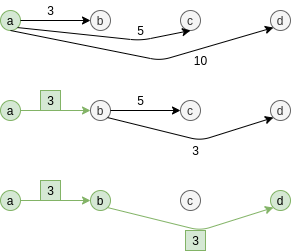
\includegraphics[max size={\textwidth}{\textheight}]{greedy-example}
    \centering
    \caption{Exemple algorisme Greedy}
    \label{fig:example-greedy}
\end{figure}


\subsection{Cost algorisme}
\subsubsection{Iteratiu}
Veiem que el programa té 3 bucles anidats\footnote{1 bucle per a recòrrer tots els punts, 1 bucle per agafar el punt de mínim cost entre un punt i el final i 1 bucle per comprovar si el arc és vàlid}
on cadascun té un pitjor cas amb cost de $O(n)$, i que en el pitjor dels casos haurem recorregut $n^3$ vegades.
Per tant, podem dir que el cost de l'algorisme en forma iterativa és de $O(n^{3})$.


\subsubsection{Recursiu}
Òbviament, si l'únic que hem fet ha sigut passar l'algorisme iteratiu a recursiu (o a l'inversa), el cost d'aquest continuarà sent el mateix. L'únic que canviarà serà que ara s'utilitzarà memòria de la pila d'execució i no memòria de heap, per tant el programa es més propens a sofrir un \textit{stackoverflow}. Finalment podem dir que el cost és de $O(n^{3})$.

\subsubsection{Empíric}
Un cop executat varies vegades l'algorisme amb un conjunt de $n$ diferents, ens crea la gràfica de la figura \ref{fig:greedy-benchmark}. Aquesta, concorda amb la justificació de la notació assimptòtica donada anteriorment.
\begin{figure}[!hbtp]
    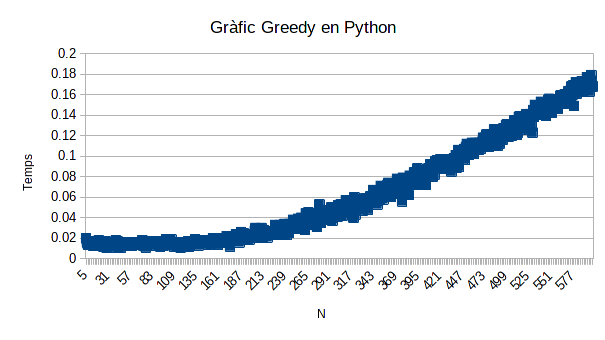
\includegraphics[max size={\textwidth}{\textheight*1/3}]{greedy-benchmark}
    \centering
    \caption{Cost empíric emprant Greedy en Python}
    \label{fig:greedy-benchmark}
\end{figure}

\subsection{Pseudo-codi de l'algorisme}
\begin{python}
def get_minimum_aqueduct():
    current_point = 0
    accumulator = cost_support(current_point)
    while current_point != final_point:
        cost, current_point = get_minimum_arch(current_point)
        if cost == infinity:
            return infinity
        accumulator = accumulator + cost
    return accumulator

def get_minimum_arch(current_point):
    # returns the minimum cost (and the point who achieves it) from current_point
\end{python}

\newpage
    
% backtracking
\section{Backtracking}
La técnica de Bactracking consisteix en anar provant totes les diferents solucions i quedar-se amb la més òptima. Una
resolució mitjançant backtracking per anar del punt A al punt D on es pot crear arcs entre tots els punts sería la figura \ref{exemple:backtracking}.

\begin{figure}[htbp]
\begin{center}
\begin{tikzpicture}[roundnode/.style={circle, draw=black!60, very thick, minimum size=7mm},]
    % nodes
    \node[roundnode]      (A)                                            {A};
    \node[roundnode]      (B1)       [below left=1cm and 4cm of A]       {B};
    \node[roundnode]      (C1)       [below =1cm of A]                   {C};
    \node[roundnode]      (D1)       [below right=1cm and 4cm of A]      {D};
    \node[roundnode]      (C2)       [below left=1cm and 2cm of B1]      {C};
    \node[roundnode]      (D2)       [below right=1cm and 2cm of B1]     {D};
    \node[roundnode]      (D3)       [below=1cm of C2]                   {D};
    \node[roundnode]      (D4)       [below=1cm of C1]                   {D};
    % lines
    \draw[->] (A.south) -- (B1.north);
    \draw[->] (A.south) --(C1.north);
    \draw[->] (A.south) --(D1.north);
    \draw[->] (B1.south) -- (C2.north);
    \draw[->] (B1.south) --(D2.north);
    \draw[->] (C2.south) --(D3.north);
    \draw[->] (C1.south) --(D4.north);
\end{tikzpicture}
\caption{Exemple crides recursives Backtracking}
\label{exemple:backtracking}
\end{center}
\end{figure}

\subsection{Cost algorisme}

\subsubsection{Recursiu}
Primerament es va tindre en compte quin sería el cost de les crides recursives que, tal i com s'aprecia a la figura \ref{figure:backtracking-nodes}, veiem que creen una forma d'arbre que haurem de recòrrer de forma postordre (finalitzem primer subarbre esquerra, després dret i finalment l'arrel). \\

Finalment, veiem que el nombre de nodes a recòrrer en funció de $n$ (on $n$ és el nombre de pilars) serà $2^{n-1}$.\\
\newpage

\begin{figure}[h!]
    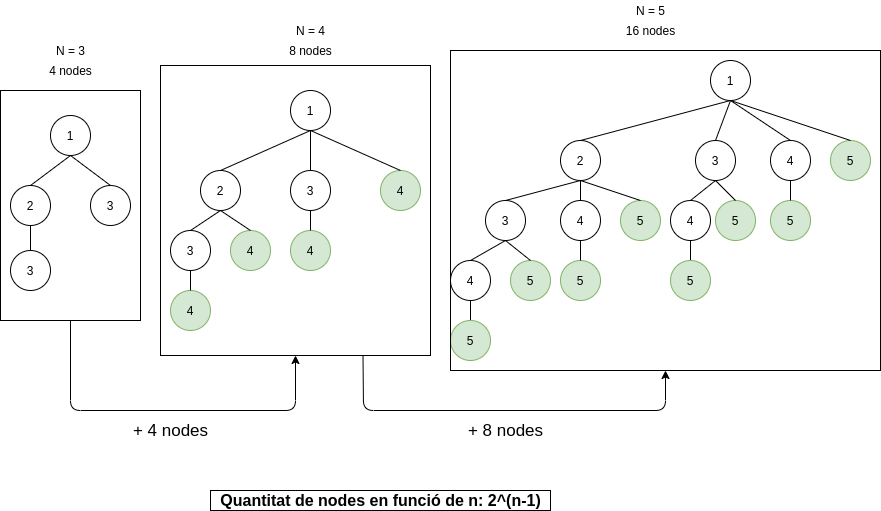
\includegraphics[max size={\textwidth}{\textheight}]{backtracking-number-nodes}
    \centering
    \caption{Nombre de nodes a les crides recursives de backtracking}
    \label{figure:backtracking-nodes}
\end{figure}

A més, falta calcular el cost de la funció $is\_valid$ en l'arbre recursiu (figura \ref{figure:backtracking-is-valid}). Aquest s'ha trobat calculant quantes vegades iterava el bucle en funció de $n$, i s'ha vist que es creava la seqüència 4, 11, 26, 57, 120, etc. S'ha deduït i comprovat que l'equació de recurrència en funció de $n$ és $2^{n-1} - n$. \\

\begin{figure}[h!]
    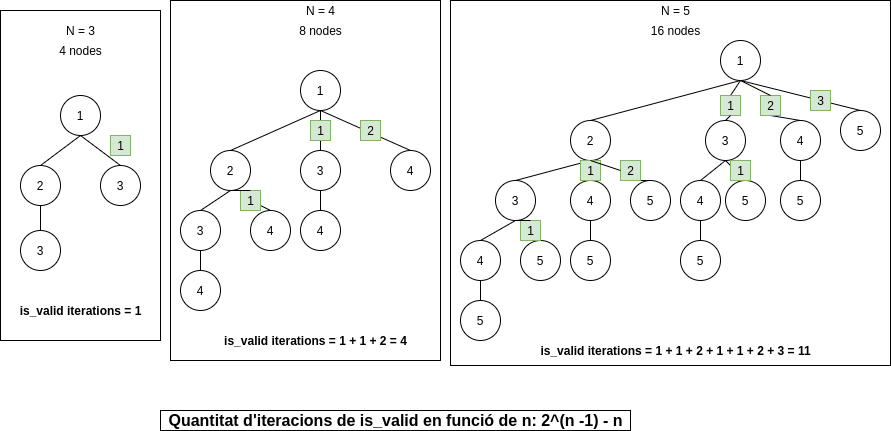
\includegraphics[max size={\textwidth}{\textheight}]{backtracking-is_valid}
    \centering
    \caption{Nombre d'iteracions de la funció is\_valid a backtracking}
    \label{figure:backtracking-is-valid}
\end{figure}

Finalment, un cop ja calculades les dos equacions de recurrència, podem sumar-les per obtenir el cost del algorisme, el que ens donaría:
\begin{center}
$2^{n-1} + 2^{n-1} - n \Longrightarrow 2*2^{n-1} - n$
\end{center}

Que en notació assimptòtica, podem representar com: $O(2^{n})$

\subsubsection{Iteratiu}
La forma més senzilla de pasar un algorisme que utilitza backtracking a iteratiu és mitjançant l'ús d'una pila\footnote{"Imitant" en certa forma el que fa la pila d'execució}. El cost algorímic serà igualment $O(2^n)$, però ara s'utilitzarà memòria de heap i no de pila d'execució, per tant \textbf{NO} es probable que sofrim un \textit{stackoverflow}.

\subsubsection{Empíric}
Finalment, s'ha executat múltiples vegades el algorisme i s'ha aconseguit formar la gràfica de la figura \ref{fig:backtracking-benchmark}, que concorda amb la nostra afirmació de que el cost és de $O(2^n)$.

\begin{figure}[!hbtp]
    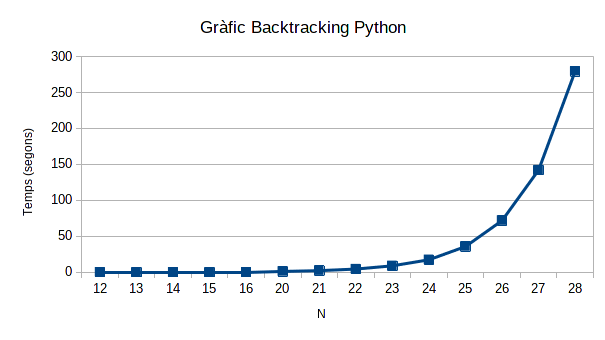
\includegraphics[max size={\textwidth}{\textheight*1/3}]{backtracking-benchmark}
    \centering
    \caption{Cost empíric emprant Backtracking en Python}
    \label{fig:backtracking-benchmark}
\end{figure}

\subsection{Pseudo-codi de l'algorisme}
\begin{python}
def get_minimum_aqueduct(current_point_index=0):
    # base case
    if current_point_index == final_point_of_aqueduct:
        return cost_support(current_point_index)
    # backtrack
        min_cost = infinity
        for analized_point from current_point_index + 1 to final_point_index:
            if valid_arch(current_point_index, analized_point):
                cost_of_analized = self.get_minimum_aqueduct(i)
                cost_of_analized += cost_support(current_point_index)
                cost_of_analized += cost_arch(current_point_index, analized_point)
                min_cost = min(min_cost, cost_of_analized)
        return min_cost
\end{python}
\newpage

% dynamic

\section{Dynamic Programming}
\label{optimal-explanation}
Abans de poder comentar la solució, hem d'entendre que és el principi d'optimitat: 
\begin{quote}{Richard E.Bellman} Principi d'optimitat: Una política òptima té la propietat que sigui quin sigui l'estat inicial i la decisió inicial, les decisions restants han de construir una política òptima respecte a l'estat resultat de la primera decisió.
\end{quote}

Per tant, seguint aquesta definició podem dir que un problema podrà ser resolt seguint el principi d'optimitat si la seva solució òptima pot ser construïda eficientment a partir de les solucions òptimes dels seus subproblemes. En altres paraules, que podem resoldre un problema gran donades les solucions dels seus problemes petits.

% nostre cas d'us
\subsection{Aplicació i funcionament en el nostre cas d'ús}
\label{seccio:funcionament}
En el nostre problema dels aqüeductes, veiem que podem aplicar el principi d'optimitat per a trobar una solució òptima, ja que la solució és construïda eficientment a partir de les solucions òptimes dels seus subproblemes. Per a explicar-ho millor he decidit resoldre un petit exemple.


Donada la següent entrada: 


\begin{center}
\begin{figure}[htbp]
\begin{CenteredBox}
\begin{lstlisting}[language={}]
5 6 180 20
0 0
2 2
3 1
5 3
7 2
\end{lstlisting}
\end{CenteredBox}
\caption{Entrada exemple}
\label{demostracio:entradaexemple}
\end{figure}
\end{center}


On podem veure que tenim 5 punts, una altura d'aqüeducte de 6, $\alpha$ = 180 i $\beta$ = 20. Si ho representem en un eix de coordenades, el perfil del sòl ens queda com la figura \ref{grafic:exemplecoordenades}, en canvi, si ho volem examinar en forma de dígraf (ja descartant opcions que no són vàlides) ens queda com a resultat la figura \ref{grafic:digraf}\\


\begin{figure}[htbp]
\begin{center}
\begin{tikzpicture}
   \tkzInit[xmax=7,ymax=6,xmin=0,ymin=0]
   \tkzGrid
   \tkzAxeXY
   \draw[thick] (0,0) -- (2, 2); 
   \draw[thick] (2,2) -- (3, 1); 
   \draw[thick] (3,1) -- (5, 3); 
   \draw[thick] (5,3) -- (7, 2); 
   \draw[thick, red] (0,6) -- (7, 6) node[midway, above] {height (6)}; 
    \foreach \Point/\PointLabel in {(0,0)/A, (2,2)/B, (3,1)/C, (5,3)/D, (7,2)/E}
   \draw[fill=black] \Point circle (0.05) node[above] {$\PointLabel$};
  \end{tikzpicture}
\caption{Exemple representat eix de coordenades}
\label{grafic:exemplecoordenades}
\end{center}
\end{figure}

\begin{figure}[htbp]
\begin{center}
\begin{tikzpicture}[roundnode/.style={circle, draw=black!60, very thick, minimum size=7mm},]
    % nodes
    \node[roundnode]      (A)                              {A};
    \node[roundnode]      (B)       [right=2cm of A]       {B};
    \node[roundnode]      (C)       [right=2cm of B]       {C};
    \node[roundnode]      (D)       [right=2cm of C]       {D};
    \node[roundnode]      (E)       [right=2cm of D]       {E};
    % lines
    \draw[->] (A.east) -- (B.west);
    \draw[->] (A.east) to[out=20,in=130] (C);
    \draw[->] (A.east) to[out=50,in=140] (D);
    \draw[->] (A.east) to[out=80,in=160] (E);
    \draw[->] (B.east) -- (C.west);
    \draw[->] (B.east) to[out=-20,in=-130] (D);
    \draw[->] (B.east) to[out=-50,in=-140] (E);
    \draw[->] (C.east) -- (D.west);
    \draw[->] (C.east) to[out=-20,in=-130] (E.west);
    \draw[->] (D.east) -- (E.west);
\end{tikzpicture}
\caption{Exemple representat en forma de dígraf}
\label{grafic:digraf}
\end{center}
\end{figure}

A continuació, anomenarem la funció $f(x)$ com el mínim cost per anar al node E. En el cas d'estar al propi node E, aquesta funció retornarà 0 (figura \ref{resultat:fdeE}).\\

\begin{figure}[htbp]
\begin{center}
\begin{tikzpicture}[roundnode/.style={circle, draw=black!60, very thick, minimum size=7mm},
                    donenode/.style={circle, draw=green!60, fill=green!5, very thick, minimum size=7mm},]
    % nodes
    \node[roundnode]      (A)                              {A};
    \node[roundnode]      (B)       [right=2cm of A]       {B};
    \node[roundnode]      (C)       [right=2cm of B]       {C};
    \node[roundnode]      (D)       [right=2cm of C]       {D};
    \node[donenode]      (E)       [right=2cm of D, label=below:$f(E)$ -> 0]       {E};
    % lines
    \draw[->] (A.east) -- (B.west);
    \draw[->] (A.east) to[out=20,in=130] (C);
    \draw[->] (A.east) to[out=50,in=140] (D);
    \draw[->] (A.east) to[out=80,in=160] (E);
    \draw[->] (B.east) -- (C.west);
    \draw[->] (B.east) to[out=-20,in=-130] (D);
    \draw[->] (B.east) to[out=-50,in=-140] (E);
    \draw[->] (C.east) -- (D.west);
    \draw[->] (C.east) to[out=-20,in=-130] (E.west);
    \draw[->] (D.east) -- (E.west);
\end{tikzpicture}
    \caption{resultat de $f(E)$}
\label{resultat:fdeE}
\end{center}
\end{figure}


En el cas de $f(D)$, únicament té una opció possible, anar del node D a F, per tant el cost mínim serà el recorregut mostrat a la figura \ref{resultat:fdeD} i la funció retornarà el valor del cost de crear un pilar a D, més el cost de crear un pilar a F i el cost de crear el arc de D a F.\\


\begin{figure}[htbp]
\begin{center}
\begin{tikzpicture}[roundnode/.style={circle, draw=black!60, very thick, minimum size=7mm},
                    donenode/.style={circle, draw=green!60, fill=green!5, very thick, minimum size=7mm},]
    % nodes
    \node[roundnode]      (A)                              {A};
    \node[roundnode]      (B)       [right=2cm of A]       {B};
    \node[roundnode]      (C)       [right=2cm of B]       {C};
    \node[donenode]      (D)       [right=2cm of C, label=below:$f(D)$ -> 1340]       {D};
    \node[donenode]      (E)       [right=2cm of D, label=below:$f(E)$ -> 0]       {E};
    % lines
    \draw[->] (A.east) -- (B.west);
    \draw[->] (A.east) to[out=20,in=130] (C);
    \draw[->] (A.east) to[out=50,in=140] (D);
    \draw[->] (A.east) to[out=80,in=160] (E);
    \draw[->] (B.east) -- (C.west);
    \draw[->] (B.east) to[out=-20,in=-130] (D);
    \draw[->] (B.east) to[out=-50,in=-140] (E);
    \draw[->] (C.east) -- (D.west);
    \draw[->] (C.east) to[out=-20,in=-130] (E.west);
    \draw[->, green] (D.east) -- (E.west);
\end{tikzpicture}
    \caption{resultat de $f(D)$}
\label{resultat:fdeD}
\end{center}
\end{figure}


En el cas de $f(C)$, té l'opció d'anar a D o d'anar a E. En aquest cas calcularem el cost de C a E i el cost de C a D + $f(D)$ i agafarem el mínim. Calculem cost de C a E i ens dona 1940, en canvi, el cost de C a D + $f(D)$ ens dona 2320. Per tant, el cost mínim des de C serà anant de C a E (figura \ref{resultat:fdeC}).\\

\begin{figure}[htbp]
\begin{center}
\begin{tikzpicture}[roundnode/.style={circle, draw=black!60, very thick, minimum size=7mm},
                    donenode/.style={circle, draw=green!60, fill=green!5, very thick, minimum size=7mm},]
    % nodes
    \node[roundnode]      (A)                              {A};
    \node[roundnode]      (B)       [right=2cm of A]       {B};
    \node[donenode]      (C)       [right=2cm of B, label=below:$f(C)$ -> 1940]       {C};
    \node[donenode]      (D)       [right=2cm of C, label=below:$f(D)$ -> 1340]       {D};
    \node[donenode]      (E)       [right=2cm of D, label=below:$f(E)$ -> 0]       {E};
    % lines
    \draw[->] (A.east) -- (B.west);
    \draw[->] (A.east) to[out=20,in=130] (C);
    \draw[->] (A.east) to[out=50,in=140] (D);
    \draw[->] (A.east) to[out=80,in=160] (E);
    \draw[->] (B.east) -- (C.west);
    \draw[->] (B.east) to[out=-20,in=-130] (D);
    \draw[->] (B.east) to[out=-50,in=-140] (E);
    \draw[->, green] (C.east) to[out=-20,in=-130] (E.west);
    \draw[->, green] (D.east) -- (E.west);
\end{tikzpicture}
    \caption{resultat de $f(C)$}
\label{resultat:fdeC}
\end{center}
\end{figure}

En el cas de $f(B)$, farem el mateix que amb $f(C)$. Calcularem quant val el cost de B a E, de B a C + $f(C)$ i de B a D + $f(D)$ i agafarem el mínim. En aquest cas el mínim es de B a E (1940) (figura \ref{resultat:fdeB}).\\

\begin{figure}[htbp]
\begin{center}
\begin{tikzpicture}[roundnode/.style={circle, draw=black!60, very thick, minimum size=7mm},
                    donenode/.style={circle, draw=green!60, fill=green!5, very thick, minimum size=7mm},]
    % nodes
    \node[roundnode]      (A)                              {A};
    \node[donenode]      (B)       [right=2cm of A, label=below:$f(B)$ -> 1940]       {B};
    \node[donenode]      (C)       [right=2cm of B, label=below:$f(C)$ -> 1940]       {C};
    \node[donenode]      (D)       [right=2cm of C, label=below:$f(D)$ -> 1340]       {D};
    \node[donenode]      (E)       [right=2cm of D, label=below:$f(E)$ -> 0]       {E};
    % lines
    \draw[->] (A.east) -- (B.west);
    \draw[->] (A.east) to[out=20,in=130] (C);
    \draw[->] (A.east) to[out=50,in=140] (D);
    \draw[->] (A.east) to[out=80,in=160] (E);
    \draw[->, green] (B.east) to[out=-50,in=-140] (E);
    \draw[->, green] (C.east) to[out=-20,in=-130] (E.west);
    \draw[->, green] (D.east) -- (E.west);
\end{tikzpicture}
    \caption{resultat de $f(B)$}
\label{resultat:fdeB}
\end{center}
\end{figure}


Finalment, en el cas de $f(A)$, haurem de calcular el cost de A a E, de A a B + $f(B)$, de A a C + $f(C)$ i de A a D + $f(D)$ i agafar el mínim cost. En aquest cas el mínim es de A a E (2780) (figura \ref{resultat:final})


\begin{figure}[htbp]
\begin{center}
\begin{tikzpicture}[roundnode/.style={circle, draw=black!60, very thick, minimum size=7mm},
                    donenode/.style={circle, draw=green!60, fill=green!5, very thick, minimum size=7mm},]
    % nodes
    \node[donenode]      (A)       [label=below:\textbf{$f(A)$ -> 2780}]                       {A};
    \node[donenode]      (B)       [right=2cm of A, label=below:$f(B)$ -> 1940]       {B};
    \node[donenode]      (C)       [right=2cm of B, label=below:$f(C)$ -> 1940]       {C};
    \node[donenode]      (D)       [right=2cm of C, label=below:$f(D)$ -> 1340]       {D};
    \node[donenode]      (E)       [right=2cm of D, label=below:$f(E)$ -> 0]          {E};
    % lines
    \draw[->, green] (A.east) to[out=20,in=160] (E);
    \draw[->, green] (B.east) to[out=-50,in=-140] (E);
    \draw[->, green] (C.east) to[out=-50,in=-130] (E.west);
    \draw[->, green] (D.east) -- (E.west);
\end{tikzpicture}
    \caption{resultat del aqüeducte mínim ($f(A)$)}
\label{resultat:final}
\end{center}
\end{figure}

% demostració algorisme
\newpage
\subsection{Demostració per reducció al absurd}
Donat un aqüeducte que va d'un punt A a un punt J i del qual sabem que el recorregut R\textsubscript{a...j} és l'òptim (figura: \ref{demostracio:atoj}).

\begin{figure}[htbp]
\begin{center}
\begin{tikzpicture}[roundnode/.style={circle, draw=green!60, fill=green!5, very thick, minimum size=7mm},]
    % nodes
    \node[roundnode]      (A)                                  {A};
    \node[roundnode]      (J)       [right=3cm of A]           {J};
    % lines
    \draw[->] (A.east) -- (J.west) node[midway, below] {R\textsubscript{a...j}};
\end{tikzpicture}
\caption{Aqüeducte de punt A a punt J}
\label{demostracio:atoj}
\end{center}
\end{figure}

Assumirem també que aquest recorregut passa per el punt K, per tant ara podem separar el recorregut com R\textsubscript{a...k} \& R\textsubscript{k...j} (figura \ref{demostracio:atoktoj})

\begin{figure}[htbp]
\begin{center}
\begin{tikzpicture}[roundnode/.style={circle, draw=green!60, fill=green!5, very thick, minimum size=7mm},]
    % nodes
    \node[roundnode]      (A)                              {A};
    \node[roundnode]      (K)        [right=3cm of A]      {K};
    \node[roundnode]      (J)        [right=3cm of K]      {J};
    % lines
    \draw[->] (A.east) -- (K.west) node[midway, below]{R\textsubscript{a...k}};
    \draw[->] (K.east) -- (J.west) node[midway, below]{R\textsubscript{k...j}};
\end{tikzpicture}
\caption{Aqüeducte de punt A a punt J passant per K}
\label{demostracio:atoktoj}
\end{center}
\end{figure}

Ara donarem com a hipòtesis que del punt A al punt K pot haver-hi un recorregut mes òptim, que anomenarem R'\textsubscript{a...k} (figura \ref{demostracio:atoktojhypotetical}).

\begin{figure}[htbp]
\begin{center}
\begin{tikzpicture}[roundnode/.style={circle, draw=green!60, fill=green!5, very thick, minimum size=7mm},]
    % nodes
    \node[roundnode]      (A)                              {A};
    \node[roundnode]      (K)        [right=3cm of A]      {K};
    \node[roundnode]      (J)        [right=3cm of K]      {J};
    % lines
    \draw[->] (A.east) -- (K.west) node[midway, below]{R\textsubscript{a...k}};
    \draw[->] (K.east) -- (J.west) node[midway, below]{R\textsubscript{k...j}};
    \draw[->, red] (A) to[out=-70,in=-100] (K) node[xshift =- 2cm, yshift =-1.8cm]{R'\textsubscript{a...k}};
\end{tikzpicture}
\caption{Graf que representa un possible R'\textsubscript{a...k}}
\label{demostracio:atoktojhypotetical}
\end{center}
\end{figure}

Si R'\textsubscript{a...k} és més òptim que R\textsubscript{a...k}, llavors vol dir que: \\
\begin{center}
R'\textsubscript{a...k} < R\textsubscript{a...k}.\\
\end{center}
Llavors:\\
\begin{center}
\textbf{R'\textsubscript{a...k} + R\textsubscript{k...j} < R\textsubscript{a...k} + R\textsubscript{k...j}} \\
\end{center}

Però aquesta afirmació \textbf{NO} pot ser certa! Ja que en un principi hem assegurat que R\textsubscript{a...k} + R\textsubscript{k...j} era la solució òptima i per tant no hi pot haver-hi cap més petita que aquesta.


\subsection{Especificació formal}
Precondició :
\begin{itemize}
    \item Una altura màxima del aqueducte (h), on ($1 \leq h \leq 10^5$)
    \item Els factors de cost $\alpha$ i $\beta$, on ($1\leq \alpha, \beta \leq 10^4$)
    \item Un conjunt de punts (x, y):\\
        $P = \{p1, p2, ... p\textsubscript{n} \mid p\textsubscript{n} = (x, y) \} \land \forall \textsubscript{x, y} \in \mathbb{N} \land n \owns \mathbb{N} \land n >= 2 
        \land x\textsubscript{i} (0\leq x\textsubscript{1} < x\textsubscript{2} < ... < x\textsubscript{n} \leq 10^5) \land y (0 \leq y\textsubscript{i} < h) $

\end{itemize}
Postcondició: cost mínim de crear l'aqueducte mitjançant els valors $\alpha$ i $\beta$ o $\infty$ en cas de que no sigui possible \footnote{Ja que tal i com es comentava a classe, havía de retornar un tipus, en aquest cas un enter o infinit. Realment en cas del programa s'ha de treure un enter si és possible o una cadena de carácters dient que és impossible}:\\

        $ resultat \in \mathbb{N} \land resultat \leq \min(R) $, on R és el conjunt de possibles resultats.


\subsection{Fòrmula algorisme}
Un cop ja sabem el funcionament del algorisme i hem demostrat que el seu comportament es correcte, podem especificar-lo amb una formula molt similar a la de l'equació de Bellman (ja que tal i com s'ha dit a la subsecció \ref{seccio:funcionament} aquest problema es resolt seguint el principi d'optimitat).

\begin{center}
\begin{equation}
v(x_{0}) = min(f(x_{0}) + v(x_{1}))
\end{equation}
On $v(x)$ és la fórmula per a calcular el cost mínim del aqüeducte, $x_{0}$ es el primer pilar del aqüeducte i $x_{1}$ es el resultat d'aplicar $v(x)$ al pilar que va desprès de $x_{0}$
\end{center}

\subsection{Cost algorisme}
\subsubsection{Iteratiu}
Veiem que el programa té 3 bucles anidats, i que en el pitjor dels casos (quan estem analitzant el primer punt, $p\textsubscript{0}$) haurem recorregut els tres $n^3$ cops.
Per tant, podem dir que el cost de l'algorisme en forma iterativa és de $O(n^{3})$.

\subsubsection{Recursiu}
Òbviament, si l'únic que hem fet ha sigut passar l'algorisme iteratiu a recursiu, el cost d'aquest continuarà sent el mateix. L'únic que canviarà serà que ara s'utilitzarà memòria de la pila d'execució i no 
memòria de heap, per tant el programa es més propens a sofrir un \textit{stackoverflow} (o \textit{recursion error} en python). Finalment podem dir que el cost és de $O(n^{3})$.

\subsubsection{Empíric}
\begin{figure}[h!]
    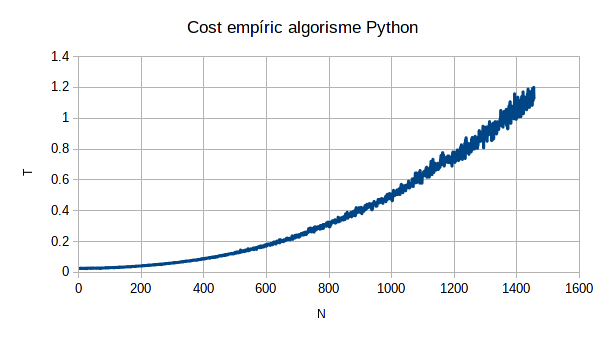
\includegraphics[max size={\textwidth}{\textheight}]{python-dynamic-benchmarks}
    \centering
    \caption{Cost empíric emprant Dynamic Programming en Python}
    \label{fig:python-dynamic-benchmarks}
\end{figure}
    
\begin{figure}[h!]
    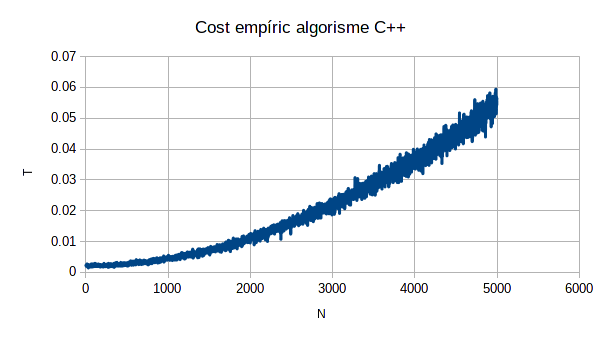
\includegraphics[max size={\textwidth}{\textheight}]{cpp-dynamic-benchmarks}
    \centering
    \caption{Cost empíric emprant Dynamic Programming en \cpluspluslogo}
    \label{fig:cpp-dynamic-benchmarks}
\end{figure}

Recalcar que en Python,  es van fer els testos fins N=1450 (figura \ref{fig:python-dynamic-benchmarks}), ja que sino el temps d'execució ja era sumament lent, mentres que 
amb \cpluspluslogo (figura \ref{fig:cpp-dynamic-benchmarks}), si que es van poder fer execucions fins N=5000.\\

Igualment, es pot apreciar que les dos gràfiques surten similar a una funció $O(n^{3})$.

\subsection{Pseudocodi algorisme}
\label{pseudocodiiteratiu}
El codi iteratiu segueix l'algorisme explicat a la secció \ref{optimal-explanation}. Recalcar que la llista que guarda els resultats és utilitzada dintre de la funció \textit{get\_minimum\_cost\_for\_index} per a no haver 
de tornar a calcular valors mínims de punts que ja havíem resolt anteriorment.

\begin{python}
def get_minimum_aqueduct():
    for i in range(self.num_points - 2, -1, -1):
        minimum_of_this_point = self.get_minimum_cost_for_index(i)
        self.point_values_buffer[i] = minimum_of_this_point
    return self.point_values_buffer[0]

def get_minimum_cost_for_index(index):
    
\end{python}

\section{Problemes al realitzar la pràctica}
\subsection{Nombres en \cpluspluslogo}
Primerament es va pensar i elaborar l'algorisme en el llenguatge de programació python, i a continuació es va migrar el codi a \cpluspluslogo. El problema va estar en no es va pensar que python al tindre tipus dinàmics el mateix intèrpret assigna un tipus a cada variable de forma intel·ligent, mentres que a \cpluspluslogo el propi programador és el que assigna els tipus. Això va generar un problema ja que, com els tests eren summament grans i podien arribar a fer operacions com per exemple $10000^{2}$, feia que no fos suficient amb els tipus integer, i s'hagués d'utilitzar tipus com per exemple ``long long int" o ``unsigned long long int".

\section{Consideracions}
\begin{enumerate}
\item Al arxiu Makefile del projecte de python, s'ha afegit una opció per a fer test del codi mitjançant l'eina pylint, però habilitant l'opció d'ignorar els ``warnings" provocats per no tindre
    comentaris per cadascún dels métodes i clases.
\item S'han mogut tots els tests a un directori anomenat \textit{test}, ja que com s'ha fet la pràctica en python y \cpluspluslogo  si no es separava s'havia de tindre els mateixos tests repetits en dos carpetes diferents.
\item S'ha decidit que el binari resultant del codi escrit en \cpluspluslogo porti habilitades les opcions d'optimització O3, ja que sinò el rendiment baixava considerablement.
\item El codi no inclou anàlisi d'errors sobre el fitxer que se li proporciona. En cas de que el format/fitxer sigui erroni, es veurà l'excepció corresponent 
    de python o \cpluspluslogo.
\item Tot i que s'ha augmentat la pila d'execució en el codi recursiu de python, recordem que la pila no és infinita i per tant en cas d'una N molt gran el programa llançarà un error de recursivitat.
\item Al programari de python s'ha emprat el patró de disseny \textit{template}, per tal de que el codi de les classes \textit{Point}, \textit{Circumference} i el \textit{parser} del fitxer no estigués repetit en 6 fitxers diferents. El fet de que python s'hagi de situar a un altre directori (anomenat \textit{common}) per poder importar els fitxers ha ocasionat afegir linees de codi que amb ulls de l'eïna pylint eren poc correctes. Aquestes s'han evitat afegint els comentaris:
    \begin{verbatim}
    # pylint: disable=wrong-import-position
    # pylint: disable=import-error
    \end{verbatim}
    per tal de poder obtenir bona puntuació a l'evaluació.
\end{enumerate}

\section{Conclusions}
Aquesta pràctica m'ha servit per adquirir els següents coneixements:
\begin{itemize}
    \item Comprendre i implementar un algorisme mitjançant backtracking.
    \item Comprendre i implementar un algorisme mitjançant greedy.
    \item Aprendre les bases de la programació funcional i veure quina millora afegíen en aquest algorisme.
    \item Iniciarme en la programació en \cpluspluslogo.
    \item Analitzar els diferents costs (empírics i teòrics) d'un algorisme.
    \item Convertir un algorisme iteratiu a recursiu.
    \item Crear un informe a partir de {\LaTeX} per a poder afegir fórmules lògiques i matemàtiques.
\end{itemize}

\newpage

\appendix

\section{Repositori github}
\label{github}

El repositori de github es pot trobar \href{https://github.com/Algorismia/Aquaeductus-Optimus}{aquí}. Recalcar que llegir el README adjuntat amb el repositori és indispensable per a saber com executar els tests de forma correcta i donarse una idea de com es troba estructurat el projecte. 

\end{document}
